\documentclass[english,14pt]{beamer}
\usetheme{EastLansing}
\usecolortheme{spruce}

\usepackage{xcolor}
\usepackage{listings}
\usepackage{courier}
\usepackage{graphicx}
\usepackage{amsmath}
\usepackage{algorithm2e}
\usepackage{multicol}
\usepackage{hyperref}
\usepackage{textcomp}

% http://mirrors.ibiblio.org/CTAN/macros/latex/contrib/datetime2/datetime2.pdf
\usepackage{babel}
\usepackage[useregional]{datetime2}

% https://tex.stackexchange.com/questions/42619/x-mark-to-match-checkmark
\usepackage{pifont}% http://ctan.org/pkg/pifont

%% https://stackoverflow.com/questions/1435837/how-to-remove-footers-of-latex-beamer-templates
%%gets rid of bottom navigation bars
%\setbeamertemplate{footline}[page number]
%
%gets rid of navigation symbols
\setbeamertemplate{navigation symbols}{}


\usefonttheme[onlymath]{serif}

\definecolor{mGreen}{rgb}{0,0.6,0}
\definecolor{mGray}{rgb}{0.5,0.5,0.5}
\definecolor{mPurple}{rgb}{0.8,0,0.82}
\definecolor{backgroundColour}{rgb}{0.95,0.95,0.92}
\definecolor{lightBlue}{rgb}{0.1, 0.1, 0.8}
\definecolor{darkGreen}{rgb}{0, 0.39, 0}

\newcommand\red[1]{{\color{red} #1}}
\newcommand\green[1]{{\color{green} #1}}
\newcommand\blue[1]{{\color{blue} #1}}
\newcommand\darkGreen[1]{{\color{darkGreen} #1}}

\newcommand{\cmark}{\ding{51}}%
\newcommand{\xmark}{\ding{55}}%

\lstdefinestyle{CStyle}{
    backgroundcolor=\color{backgroundColour},   
    commentstyle=\color{mGreen},
    keywordstyle=\color{magenta},
    numberstyle=\tiny\color{mGray},
    stringstyle=\color{mPurple},
    basicstyle=\footnotesize,
    breakatwhitespace=false,         
    breaklines=true,                 
    captionpos=b,                    
    keepspaces=true,                 
    numbers=left,                    
    numbersep=5pt,                  
    showspaces=false,                
    showstringspaces=false,
    showtabs=false,                  
    tabsize=2,
    language=Python
}

\lstdefinestyle{pseudo}{
        basicstyle=\ttfamily\footnotesize,
        keywordstyle=\color{lightBlue},
        morekeywords={BEGIN,END,IF,ELSE,ENDIF,ELSEIF,PRINT,WHILE,RETURN,ENDWHILE,DO,FOR,TO,IN,ENDFOR,BREAK,INPUT,CONDITIONS},
        morecomment=[l]{//},
        commentstyle=\color{mGreen}
}

\lstset{basicstyle=\footnotesize\ttfamily,breaklines=true}
\lstset{framextopmargin=50pt,tabsize=2}

\title{ENGG1003 - Thursday Week 9}
\subtitle{Normally distributed random numbers}
\author{Steve Weller}
\institute{University of Newcastle}
%\date{\today}
\date{6 May 2021}

% following is a bit of a hack, but forces page numbers (technically: frame numbers) to run 1,2,3,... 
% with titlepage counting as frame 1

\addtocounter{framenumber}{1}
\titlepage

\begin{document}

\begin{flushleft}
{\scriptsize Last compiled:~\DTMnow}
\vspace*{-5mm}
\end{flushleft}
\framebreak

%==============================================================

\begin{frame}[fragile]

\frametitle{Lecture overview}
\begin{enumerate}
	\item recap: uniformly distributed random numbers
	\begin{itemize}
		\item pdf of uniformly distributed rv
		\item area under pdf is probability
		\item histogram, normalized histogram is basically pdf
	\end{itemize}

	\item[]
	
	\item standard normal distribution (bell curve)
	\begin{itemize}
		\item pdf, mean $\mu = 0$ and $\sigma = 1$ %zero and std 1, 
		\item generate using Python
		\item area (needs integration) and probability
	\end{itemize}
	
%	\item[]
%	
%	\item normal distribution (aka Gaussian)
%	\begin{itemize}
%		\item pdf, meaning of $\mu$ and $\sigma$
%		\item generate using Python
%		\item area (needs integration) and probability
%	\end{itemize}
	
	\item[]
	
	\item engineering application
	
\end{enumerate}

\end{frame}

%==============================================================

\begin{frame}[fragile]

\frametitle{$1)$ Uniformly distributed random numbers}

% https://www.w3schools.com/python/python_ml_data_distribution.asp

\begin{itemize}
	\item Create an array containing 250 random floats between 0 and 5
\end{itemize}

%  random.uniform(low=0.0, high=1.0, size=None)

\texttt{filename.py}
\begin{lstlisting}[style=CStyle,basicstyle=\scriptsize]
import numpy as np

x = np.random.uniform(0.0, 5.0, 250)

print(x) 
\end{lstlisting}

\end{frame}

%==============================================================

\begin{frame}[fragile]

\frametitle{histogram}

% https://www.w3schools.com/python/matplotlib_histograms.asp

% https://www.w3schools.com/python/python_ml_data_distribution.asp

\begin{itemize}
	\item A histogram is a graph showing frequency distributions
	\item It is a graph showing the number of observations within each given interval.
	\item To visualize the data set we can draw a histogram with the data we collected
	\item We will use the Python module Matplotlib to draw a histogram
\end{itemize}

\texttt{filename.py}
\begin{lstlisting}[style=CStyle,basicstyle=\scriptsize]
import numpy as np
import matplotlib.pyplot as plt

x = np.random.uniform(0.0, 5.0, 250)

plt.hist(x, 5)
plt.show() 
\end{lstlisting}

\end{frame}

%==============================================================

\begin{frame}[fragile]

\frametitle{}

\begin{figure}[ht]
	\centering
	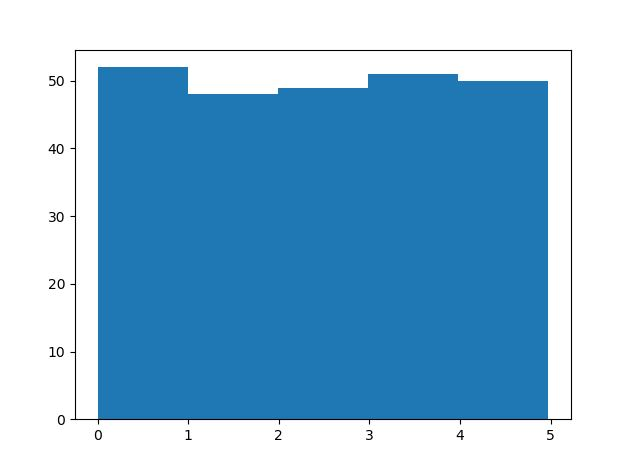
\includegraphics[width=0.8\textwidth]{figures/uniformOutput}
\end{figure}

\end{frame}

%==============================================================

\begin{frame}[fragile]

\frametitle{normalized histogram is basically pdf}

\begin{itemize}
	\item same plot as previous, but now normalize using \texttt{density=True} in \texttt{hist}
\end{itemize}

\end{frame}

%==============================================================

\begin{frame}[fragile]

\frametitle{pdf of uniformly distributed rv}

\begin{itemize}
	\item xxx
\end{itemize}

\end{frame}

%==============================================================

\begin{frame}[fragile]

\frametitle{area under pdf is probability}

\begin{itemize}
	\item xxx
\end{itemize}

\end{frame}

%==============================================================

\begin{frame}[fragile]

\frametitle{$2)$ Standard normal distribution}

\begin{itemize}
	\item xxx
\end{itemize}

\end{frame}

%==============================================================

\begin{frame}[fragile]

\frametitle{}

\begin{itemize}
	\item xxx
\end{itemize}

\end{frame}

%==============================================================

\begin{frame}[fragile]

\frametitle{}

\begin{itemize}
	\item xxx
\end{itemize}

\end{frame}

%==============================================================

\begin{frame}[fragile]

\frametitle{}

\begin{itemize}
	\item xxx
\end{itemize}

\end{frame}

%==============================================================

\begin{frame}[fragile]

\frametitle{$3)$ Engineering application}

\begin{itemize}
	\item xxx
\end{itemize}

\end{frame}


%==============================================================

\begin{frame}[fragile]

\frametitle{Lecture summary}

\begin{enumerate}
	\item xxx
	
	\item[]
	
	\item xxx
	
	\item[]
	
	\item xxx
	
	\item[]
	
	\item what's next
	
\end{enumerate}

\end{frame}

\end{document}